\chapter{Evaluation of TIDE}

\section{Experiment script}
\label{app:evalscript}

\emph{Introduction speech to the user:}
\\\\
``The experiment is divided in 3 parts.
The first part will allow you to discover the application and learn to use it.
In the second part, I will guide you through two scenarios where you will play a role, and have to do specific things with the application.
The third part is an online questionnaire that you will fill out on the computer.
\\\\
But first, let me present what we will be working with.
% PRESENT SMARTPHONES HERE !!!
This is the Microsoft Surface, a tabletop computer with a multitouch screen.
It works like a big smartphone, please try.
\\\\
We will use an application called TIDE.
This application allows you to connect a smartphone to the tabletop.

TIDE is a only a prototype, meaning that there are things that are not finished, and some that are not implemented, so please be patient in case of unexpected behavior.
Especially, please be aware of the following things:
\begin{itemize}
\item to pair the phone with the table, you place it, and the table detects it. what happens is that sometimes the table does not see the phone, so you have to move it around until it works. Sometimes the table will think it sees a new phone, so you will have to click 'no'.
\item when you touch inside the window, you interact with the phone. But the application is slow. So after every input, it is necessary to wait that the screen is updated, before giving the next input.
\item as you can see, there are two elements to the application. Inside the window is for using the phone, but you can also manipulate the window. This is what this experiment focuses on.
\item Finally, one important thing, remember that it is the system that is under test here, not you.
\end{itemize}
Let us start.''

\subsection{Discovering Tide (10 min)}

\subsubsection{Free exploration}
 
``
You have a few minutes to discover the application on your own.
Here is a list of what you can try to do with the application.
Please, comment aloud on what you are doing, and what is happening.
''

The list of suggestions should be apparent, for example hanging on the wall.

%Suggestions:
% pair the phone to the table
% move the window around
% rotate the window
% resize the window
% minimize the window
% close the window and pair again

\subsubsection{Features (designer fills out EF1)}

``
Together, we will go through all the application features, and I will teach you the features that you haven't discovered on your own.
I fill out this form, where I register which features you discovered yourself.
''

\subsection{Using Tide (10 min)}

``
Now we will do a little bit of role playing. We will go through two scenarios, where I will direct you to do specific things with the application.
I will tell you exactly what to do, step by step, but it is up to you to decide how to do it.
''

\subsubsection{Gaming}

``
The first scenario is about two friends in a waiting room. They are bored, and decide to play a game of tic-tac-toe to pass the time.
''

\begin{enumerate}
\item connect the iPhone to the tabletop
\item launch the game called 'tic tac toe'
\item start a 2 players game
\item enlarge the window and position it so we can play
\item now we play
\item exit the game
\item close the application
\end{enumerate}

\subsubsection{Browsing}

``
The second scenario is about two friends that are planning a surprise dinner for the birthday of a third friend named Bob. 
You will look up a place called cafe alma on the internet, and you will show me where it is and how to go there from here.
When Bob approaches, you should hide what we are doing.
''

\begin{enumerate}
\item connect the HTC Legend to the tabletop
\item launch the app called Internet
\item adjust the position and size of the window
\item type on the google search bar
\item type 'cafe alma' and hit search
\item tap 'contact'
\item Bob is passing by, minimize the window
\item restore the window
\item use your phone to zoom on the address
\item go back to home screen
\item launch the app called Maps
\item hit search
\item type 'isafjordsgade 5' and hit enter
\item zoom in on the address
\item find ITU on the map
\item adjust the position and size of the window to show it to me
\item Bob is here, minimize the window
\item restore the window
\item show me how to walk from ITU to cafe alma
\item return to phone home screen
\item exit application
\end{enumerate}

\subsection{Questionnaire (10 min)}

The user fills in the evaluation form Tide-EF2.

\clearpage
\section{Experiment forms}
\label{app:evalforms}

\begin{figure}[htb]
  \centering
    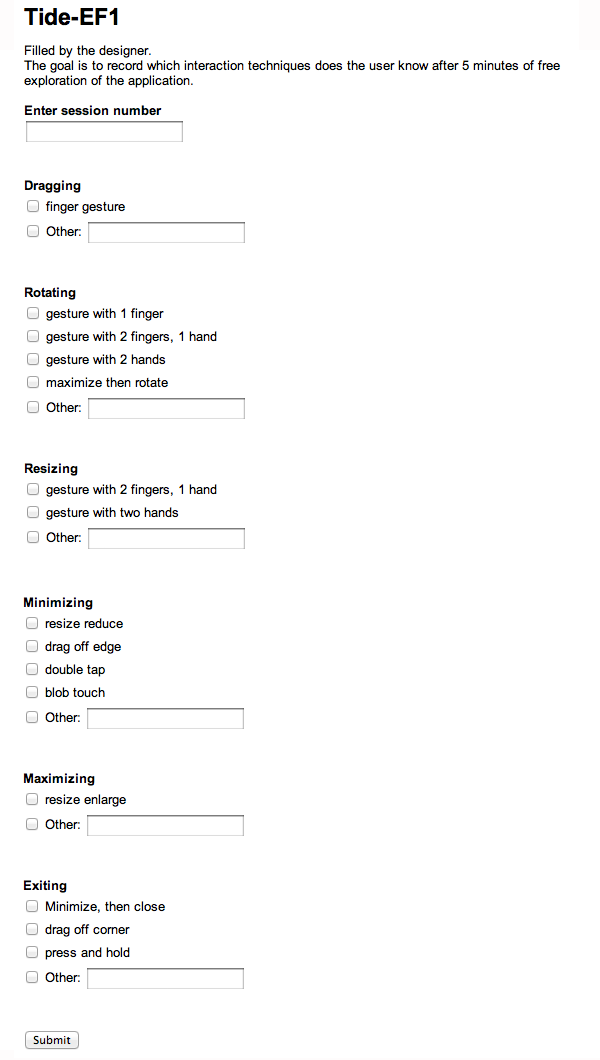
\includegraphics[width=0.7\textwidth]{images/evalform1}
    %\caption{TIDE: component diagram.}
    %\label{fig:overview}
\end{figure}

\begin{figure}[htb]
  \centering
    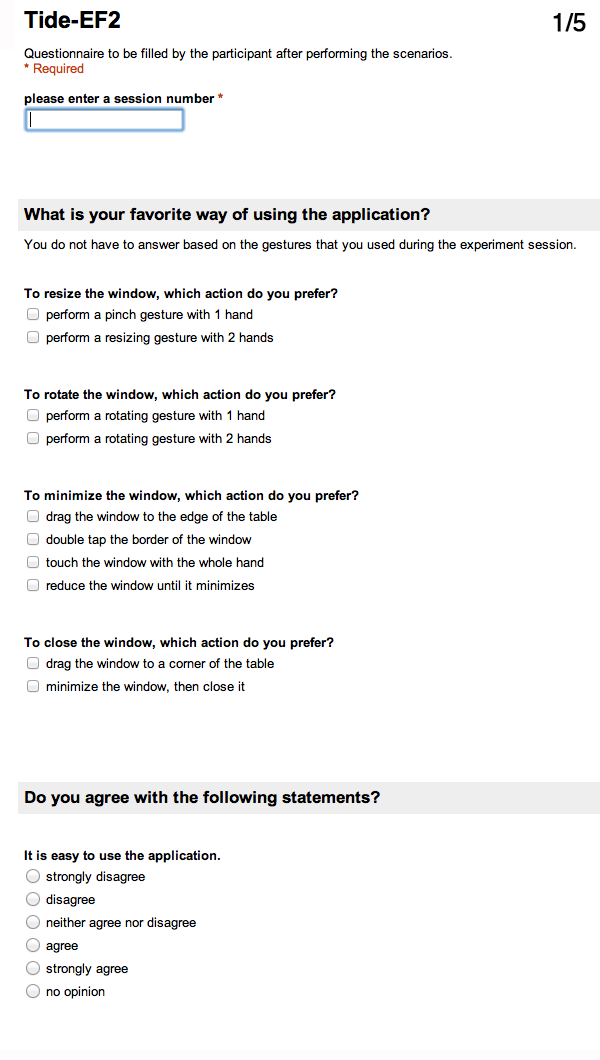
\includegraphics[width=0.8\textwidth]{images/evalform2a}
    %\caption{TIDE: component diagram.}
    %\label{fig:overview}
\end{figure}

\begin{figure}[htb]
  \centering
    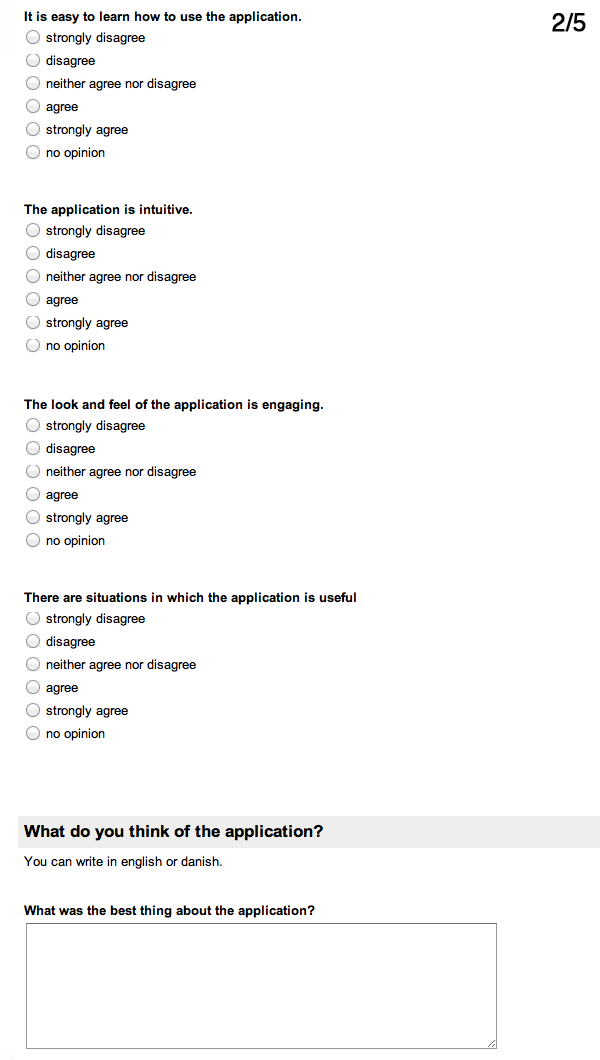
\includegraphics[width=0.8\textwidth]{images/evalform2b}
    %\caption{TIDE: component diagram.}
    %\label{fig:overview}
\end{figure}

\begin{figure}[htb]
  \centering
    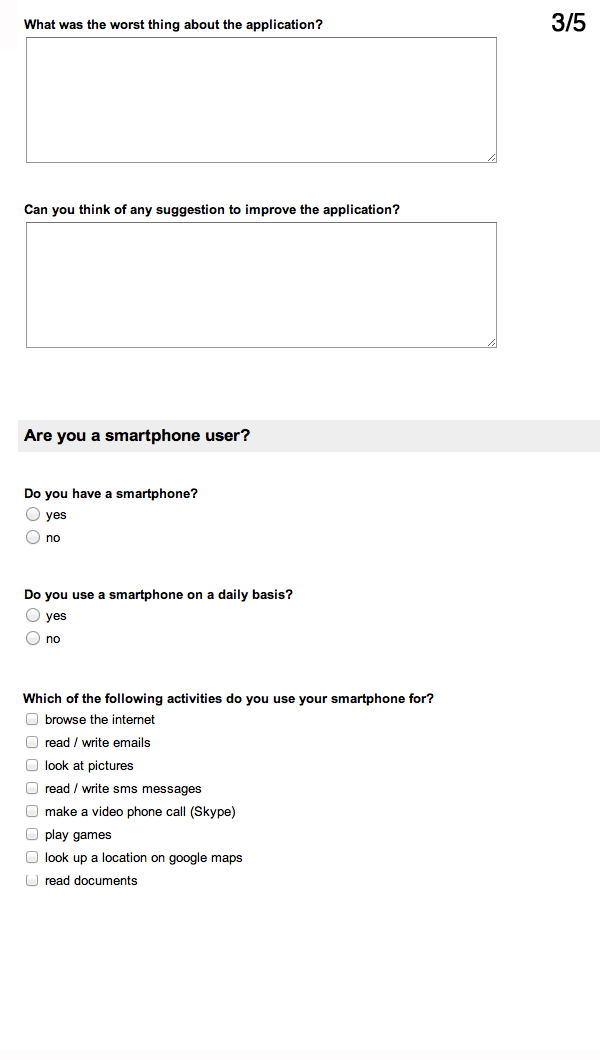
\includegraphics[width=0.8\textwidth]{images/evalform2c}
    %\caption{TIDE: component diagram.}
    %\label{fig:overview}
\end{figure}

\begin{figure}[htb]
  \centering
    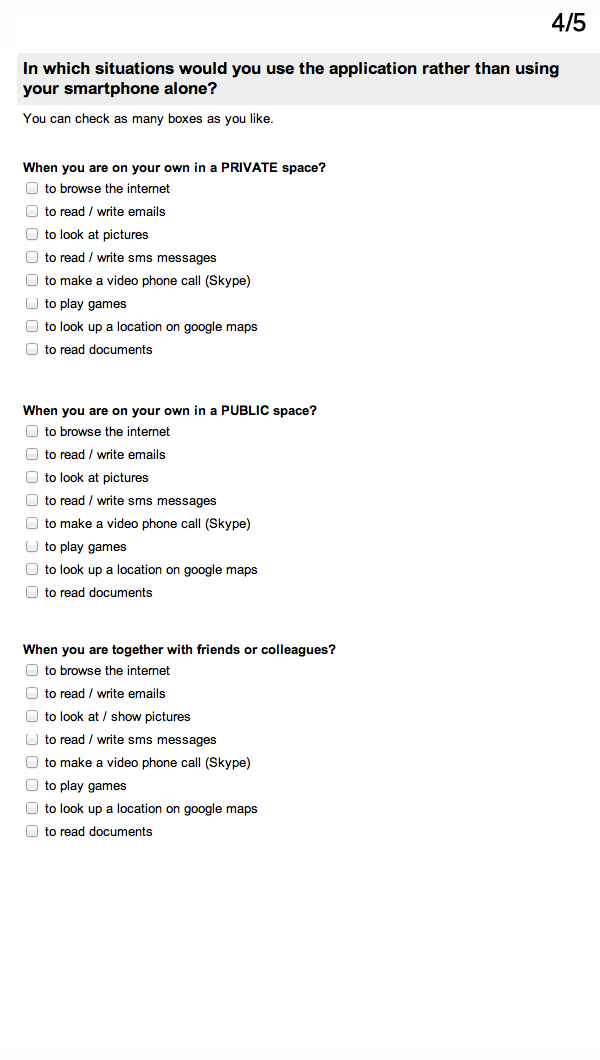
\includegraphics[width=0.8\textwidth]{images/evalform2d}
    %\caption{TIDE: component diagram.}
    %\label{fig:overview}
\end{figure}

\begin{figure}[htb]
  \centering
    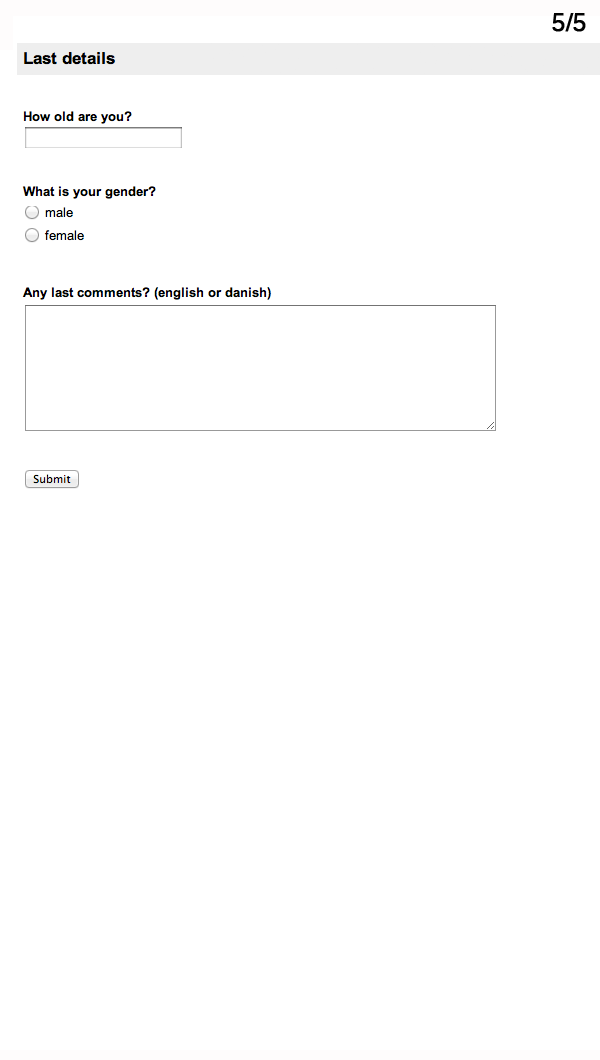
\includegraphics[width=0.8\textwidth]{images/evalform2e}
    %\caption{TIDE: component diagram.}
    %\label{fig:overview}
\end{figure}

%teaching phase for each primitive (5):
%1) ask them to do it
%	- do they know how to do it
%	- which technique do they use?
%2) ask them if they know of other technique
%- if yes, which? show?
%- if no, tell them. show?
%
%scenario phase:
%1) browsing:
%- pair Legend
%- look up sthg online: remote UI, dragging, resizing
%- shoe me sthg: rotating
%- hide stag from someone: minimizing/hiding
%
%2) gaming (designer is opponent)
%- pair iPhone
%- launch game: remote UI
%- resize to fullscreen (maximize)
%- exit
%
%questionnaire phase: google forms?
%= straightforward user satisfaction study
%- rate the experience: usable? engaging?
%- would you use such a system?
%- how intuitive is the system?
%
%
%LOGGING (user, session, command, action, timestamp)
%
%drag, resize, rotate = using active border
%
%maximize by size enlarge
%rotate when maximized
%
%minimize by drag to edge
%minimize by double tap
%minimize by blob touch
%minimize by size reduce
%
%close by minimize
%close by corner
%close by press and hold
